\documentclass[english]{achemso}
\setkeys{acs}{keywords = true, email=false}
\usepackage[T2A,LGR,T1]{fontenc}
\usepackage{babel}
\usepackage{array}
\usepackage{textcomp}
\usepackage{url}
\usepackage{multirow}
\usepackage{amsmath}
\usepackage{graphicx}
\usepackage{subscript}
%\usepackage[unicode=true,pdfusetitle,
% bookmarks=true,bookmarksnumbered=false,bookmarksopen=false,
% breaklinks=false,pdfborder={0 0 0},pdfborderstyle={},backref=false,colorlinks=false]
% {hyperref}
%\usepackage{lineno}
%\linenumbers

\makeatletter

%%%%%%%%%%%%%%%%%%%%%%%%%%%%%% LyX specific LaTeX commands.


\title{Wetting of the tarsal adhesive fluid controls underwater adhesion in ladybug beetles: Supplementary material}

\author{Pranav Sudersan}


\affiliation{Max Planck Institute for Polymer Research, Ackermannweg 10, 55128
Mainz, Germany}


\author{Michael Kappl}


\affiliation{Max Planck Institute for Polymer Research, Ackermannweg 10, 55128
Mainz, Germany}


\author{Bat-El Pinchasik}


\affiliation{School of Mechanical Engineering, Tel Aviv University, Tel Aviv-Yafo,
Israel}


\author{Hans-J\"{u}rgen Butt}


\affiliation{Max Planck Institute for Polymer Research, Ackermannweg 10, 55128
Mainz, Germany}


\author{Thomas Endlein}


\affiliation{Max Planck Institute for Polymer Research, Ackermannweg 10, 55128
Mainz, Germany}


\DeclareRobustCommand{\greektext}{%
  \fontencoding{LGR}\selectfont\def\encodingdefault{LGR}}
\DeclareRobustCommand{\textgreek}[1]{\leavevmode{\greektext #1}}
\ProvideTextCommand{\~}{LGR}[1]{\char126#1}

\DeclareRobustCommand{\cyrtext}{%
  \fontencoding{T2A}\selectfont\def\encodingdefault{T2A}}
\DeclareRobustCommand{\textcyr}[1]{\leavevmode{\cyrtext #1}}

\newcommand{\lyxmathsym}[1]{\ifmmode\begingroup\def\b@ld{bold}
  \text{\ifx\math@version\b@ld\bfseries\fi#1}\endgroup\else#1\fi}

%% Because html converters don't know tabularnewline
\providecommand{\tabularnewline}{\\}

%%%%%%%%%%%%%%%%%%%%%%%%%%%%%% User specified LaTeX commands.
\SectionNumbersOn
%\setkeys{acs}{doi = true}
\setkeys{Gin}{width=\linewidth}
\usepackage{subcaption}


\makeatother

\begin{document}
%reset figure/table/equation numbers and include prefix
\renewcommand{\thesection}{S1.\arabic{section}}
\setcounter{figure}{0} \renewcommand{\thefigure}{S1.\arabic{figure}} 
\setcounter{table}{0} \renewcommand{\thetable}{S1.\arabic{table}} 
\setcounter{equation}{0} \renewcommand{\theequation}{S1.\arabic{equation}}

\section{Simulation method: Single capillary bridge \label{subsec:Simulation-Method}}

Capillary force due to a single adhesive fluid or bubble meniscus (termed ``capillary
bridge'') is calculated by performing simulations in Surface Evolver
\cite{RN206}, similar to the method described by \citet{RN93}.
A simple cubic geometry, mimicking the capillary bridge, of constant
volume, $V$, is defined as the initial condition with an interfacial
tension, $\gamma$, with the surrounding medium. Interfacial tension
of the capillary bridge with the substrate is given by $\gamma\cos\theta$,
where $\theta$ is the corresponding contact angle inside the bridge.
For the case of a bubble meniscus, $\theta$ is defined w.r.t. the
surrounding water, since $\theta$ can also directly characterise
the substrate wettability. The capillary bridge spans a gap distance
$d$ between the top face and the substrate. The boundary conditions
are set corresponding to a pinned contact line of diameter $D$ on
the top face and constant interfacial tension with the substrate on
the bottom. All lengths are normalised relative to length $s=\left(3V/4\pi\right)^{1/3}$.
An appropriate geometry refinement routine is chosen to evolve the
capillary bridge shape to its minimum energy state. The normalised
total capillary force, $\hat{f}=f/\gamma s$, is the sum of the Laplace
pressure and surface tension contributions , where:

\begin{equation}
f=f_{laplace}+f_{surface\,tension}=\varDelta P_{laplace}A_{_{bottom}}+2\pi R_{bottom}\gamma\sin\theta\label{eq:f_bridge}
\end{equation}

Here, $\varDelta P_{laplace}$ is the Laplace pressure of the equilibrium
capillary bridge, $A_{bottom}$ is the contact area of the capillary
bridge with the substrate at bottom and $R_{bottom}$ is the corresponding
radius of contact, all obtained from the simulation output for the
equilibrium surface.

The gap distance $d$ is varied stepwise and the capillary force is
calculated each time to obtain force-distance curves for a particular
choice of $D$ and $\theta$. 

\section{Single capillary bridge: Effect of volume}

Surface Evolver simulation results showing the effect of volume on
the maximum capillary force of a single fluid bridge. Since the fluid
is pinned at the top to the same diameter, D, a smaller volume would
result in high interfacial curvatures, which increases the capillary
force due to the negative Laplace pressure. In this case, small contact
angles lead to a greater increase in adhesion.

\begin{figure}[H]

\begin{centering}
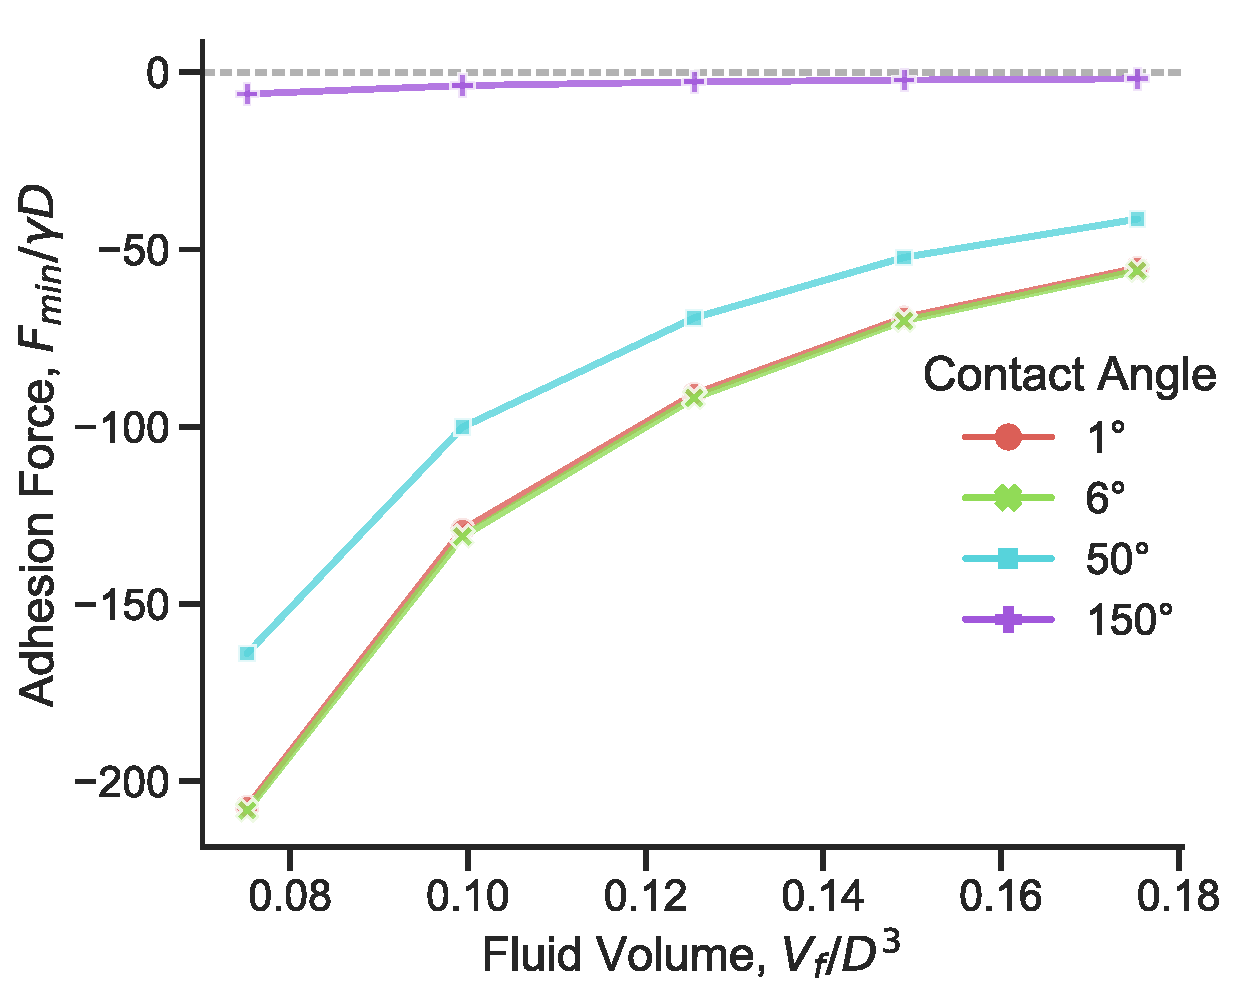
\includegraphics{FigureS2-Effect_of_fluid_volume}\caption{Normalised maximum capillary force for a single bridge as a function
of fluid volume}
\par\end{centering}
\end{figure}


\section{Capillary Bridge Model: Effect of hair diameter at constant fluid
volume}

Here, instead of scaling the fluid volume relative to the hair diameter,
we now assume a fixed total fluid volume distributed equally among
the $N$ hairs. Total fluid volume, $V_{total}=NV_{f}=2000$. Hair
diameter is varied while keeping the total hair contact area constant.
Length is in arbitrary units. Forces increase at a much smaller rate
on decreasing diameter when compared to the case with self-similar
scaling of fluid volume (Figure 8 in main text).

\begin{figure}[H]
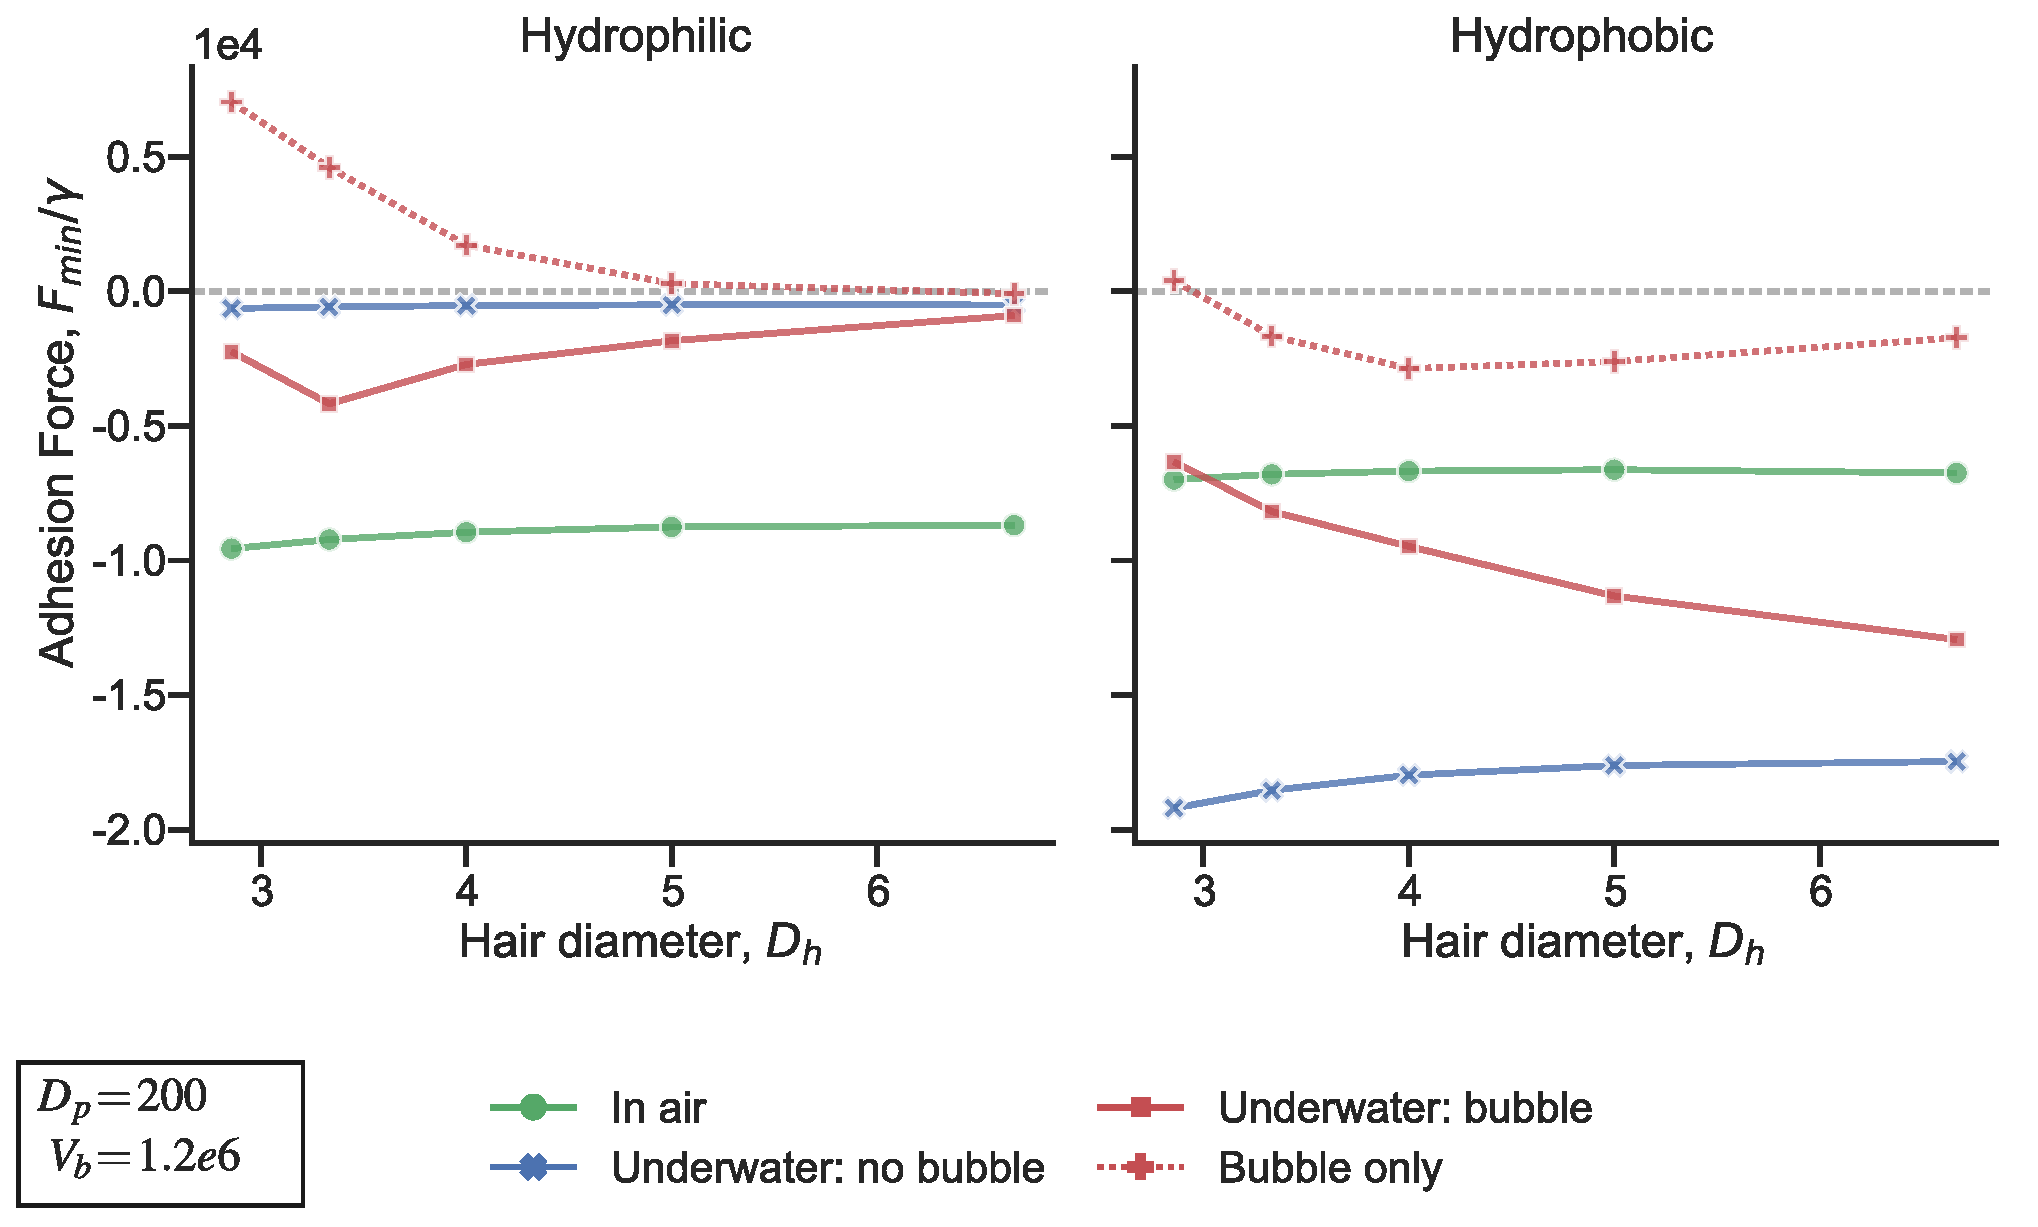
\includegraphics{FigureS3-Effect_of_hair_size(constant_vol)}

\caption{Normalised adhesion force of hairy pad system on a hydrophilic and
hydrophobic substrate as a function of hair diameter ($D_{h}$), calculated
from the capillary bridge model. The total adhesive fluid volume is
fixed to 2000. Adhesion forces are calculated from minima of the respective
force-distance curves. Negative force value represents attraction.
The bubble's contribution to the net force for an \emph{underwater:
bubble} contact is denoted by plus symbols. Bubble volume and pad
diameter are kept fixed. All lengths are scaled relative to $D_{p}$.}
\end{figure}


\section{Statistical comparison}

Pairwise statistical comparison of single leg adhesion force measurements
of the ladybug beetle (\emph{Coccinella septempuctata}) for each contact
type and substrate are shown (Table \ref{tab:Statistical-analysis}).
The uncorrected p-values and Common Language Effect Size (CLES) are
obtained from post-hoc pair-wise Student t-test between A and B while
keeping the third parameter fixed. p-values showing statistically
significant difference between A and B are in boldface. 
CLES represents the statistical proportion of samples under A with higher adhesion than under B. The condition
for statistical significance is based on the Bonferroni-corrected
critical p-value of 0.008.

\begin{table}[H]
\noindent \begin{centering}
\begin{tabular}{|>{\raggedright}m{0.15\linewidth}|>{\raggedright}m{0.15\linewidth}|>{\raggedright}m{0.15\linewidth}|>{\centering}m{0.15\linewidth}|>{\centering}m{0.15\linewidth}|}
\hline 
Fixed & A & B & p-value & CLES\tabularnewline
\hline 
\hline 
In air & PFOTS & Glass & 0.959 & 0.48\tabularnewline
\hline 
Underwater: bubble & PFOTS & Glass & 0.011 & 0.96\tabularnewline
\hline 
Underwater: no bubble & PFOTS & Glass & \textbf{< 0.001} & 1.0\tabularnewline
\hline 
PFOTS & In air & Underwater: bubble & 0.897 & 0.48\tabularnewline
\hline 
PFOTS & In air & Underwater: no bubble & 0.828 & 0.48\tabularnewline
\hline 
PFOTS & Underwater: bubble & Underwater: no bubble & 0.721 & 0.44\tabularnewline
\hline 
Glass & In air & Underwater: bubble & \textbf{0.002} & 1.0\tabularnewline
\hline 
Glass & In air & Underwater: no bubble & \textbf{< 0.001} & 1.0\tabularnewline
\hline 
Glass & Underwater: bubble & Underwater: no bubble & 0.07 & 0.84\tabularnewline
\hline 
\end{tabular}
\par\end{centering}
\caption{\label{tab:Statistical-analysis}}
\end{table}


\section{Field desorption mass spectroscopy}

To test whether the ladybug beetles retain
their adhesive fluid underwater unchanged, we performed a Field Desorption Mass Spectroscopy
(FDMS) using a ZAB 2-SE-FPD spectrometer (VG Instruments, Malaysia). The measurements
were done on the extracted secretions before and after submerging its
legs under water. The middle leg of an Asian ladybird (\emph{Harmonia
axyridis}) was immersed in 50 \textmu L Tetrahydrofuran (THF) for 20 min and then transferred
to the measurement chamber of the FDMS. As a reference, pure THF was
used. The second middle leg of the same ladybird was subsequently
immersed in 100 \textmu L Milli-Q water for 15 min (close to the time-scale of the underwater adhesion tests), then in THF for
20 min and then transferred to the measurement chamber of the spectrometer.
Molecular weights were extracted from the peak positions of the
FDMS spectra. Probable compostion was identified from the molecular weights by assuming the secretion fluid consists possibly of hydrocarbons, alcohols, aldehydes or carboxylic acids.

FDMS results confirm the presence of adhesive fluid on the Asian ladybird's
leg when underwater (Table \ref{tab:Molecular-distribution-of}).
Molecular weights of the epicuticular grease extracted from the beetle’s leg, without and after immersion in water, show that, except
for two molecular weights (406.8 g mol\protect\textsuperscript{-1} and 331.6 g mol\protect\textsuperscript{-1}), the chemical
fingerprint remained unchanged. This let us assume that the tarsal adhesive fluid
was not washed away underwater. Probable compounds in the fluid, corresponding
to the resultant molecular weights, include mostly aliphatic hydrocarbons
with traces of aldehydes. Our preliminary measurements on \emph{Harmonia axyridis} let us conjecture that, 
even for the case of \emph{Coccinella septempuctata}, the tarsal adhesive fluid was not washed away from the hairs during the underwater experiments. A detailed study is however essential to ensure that the difference in the ladybug species between our adhesion and FDMS tests doesn't qualitatively change the above outcome. Further, the detected compounds would also include cuticular secretions from the leg apart from the tarsal fluid. Thus, a more precise fluid extraction method is necessary to definitely confirm the above conjecture, and will be a subject of future study.

\begin{table}[H]
\centering{}%
\begin{tabular}{|c|c|c|}
\hline 
Without submerging (g mol\protect\textsuperscript{-1}) & After submerging (g mol\protect\textsuperscript{-1}) & Probable compounds\tabularnewline
\hline 
\hline 
324.5 & 324.5 & C\textsubscript{23}H\textsubscript{48}, C\textsubscript{22}H\textsubscript{44}O\tabularnewline
\hline 
 & 331.6 & C\textsubscript{24}H\textsubscript{44}\tabularnewline
\hline 
350.5 & 350.5 & C\textsubscript{25}H\textsubscript{50}\tabularnewline
\hline 
352.5 & 352.5 & C\textsubscript{25}H\textsubscript{52}, C\textsubscript{24}H\textsubscript{48}O\tabularnewline
\hline 
378.5 & 378.5 & C\textsubscript{27}H\textsubscript{54}\tabularnewline
\hline 
404.6 & 404.5 & C\textsubscript{29}H\textsubscript{56}\tabularnewline
\hline 
406.8 &  & C\textsubscript{29}H\textsubscript{58}\tabularnewline
\hline 
432.8 & 432.7 & C\textsubscript{31}H\textsubscript{60}\tabularnewline
\hline 
\end{tabular}\caption{Molecular weights of the tarsal adhesive fluid secretion of \emph{Harmonia axyridis}
without and after submerging the beetle's leg in water. \label{tab:Molecular-distribution-of}}
\end{table}


\section{Capillary force due to a bubble\label{subsec:Capillary-force-due}}

Capillary force of a single bubble against a PFOTS surface are compared
for two different volumes. The volumes correspond to the expected
range in the case of the trapped bubble in a ladybug. Here, the bubble
is pinned to a micropatterned PDMS substrate on the top. The maximum
adhesion force of any of the bubble never exceeds 50 \textmu N,
significantly lower than the beetle's underwater adhesion to the same
substrate (> 400 \textmu N). Thus, the bubble's contribution
to adhesion in the ``\emph{underwater: bubble}'' contact of a ladybug's
pad should be negligible. Measurement videos are included in the supplementary material (S6).

\begin{figure}[H]
\begin{centering}
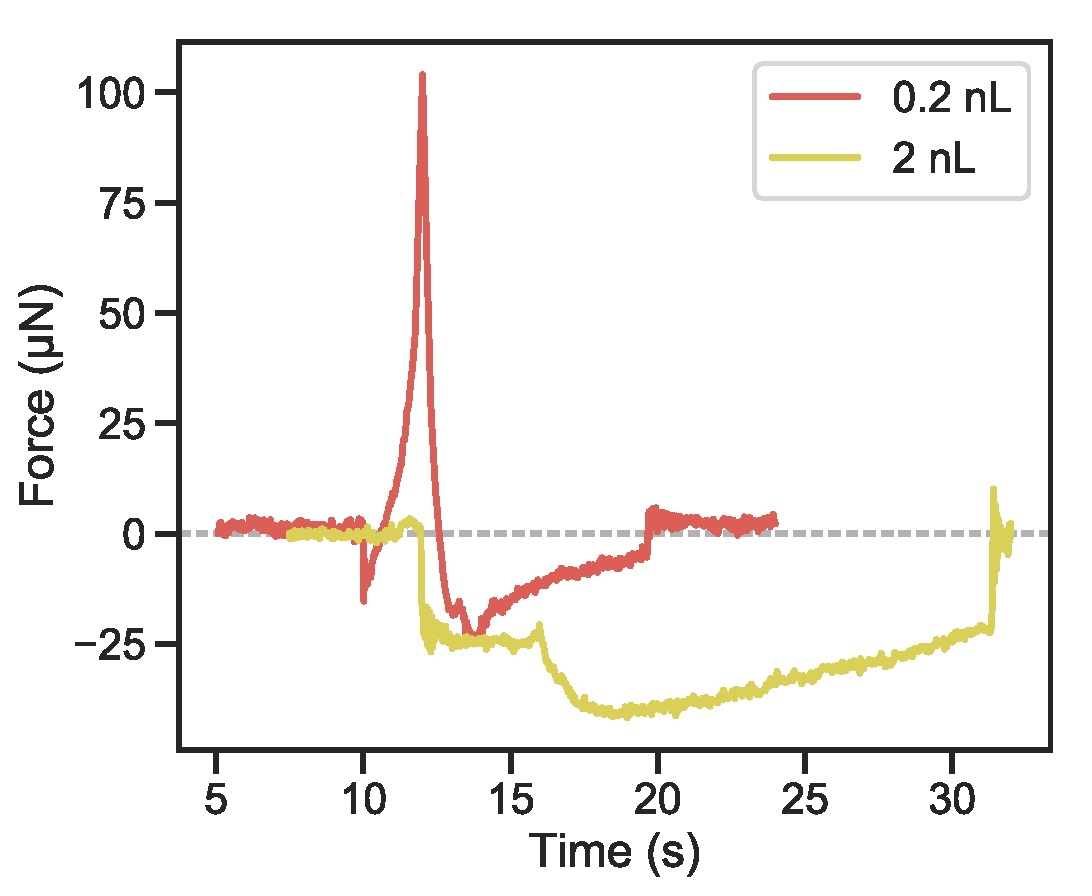
\includegraphics{FigureS4-Expt_bubble_force}\caption{Capillary force of the bubble}
\par\end{centering}
\end{figure}

\bibliography{references}

\end{document}